%%%%%%%%%%%%%%%%%%%%%%%%%%%%%%%%%%%%%%%%%
% APA Assignment Article
% LaTeX Template
% Version 2.0 (February 7, 2023)
%
% This template originates from:
% https://www.LaTeXTemplates.com
%
% Author:
% Vel (vel@latextemplates.com)
%
% License:
% CC BY-NC-SA 4.0 (https://creativecommons.org/licenses/by-nc-sa/4.0/)
%
% NOTE: The bibliography needs to be compiled using the biber engine.
%
%%%%%%%%%%%%%%%%%%%%%%%%%%%%%%%%%%%%%%%%%

%----------------------------------------------------------------------------------------
%	PACKAGES AND OTHER DOCUMENT CONFIGURATIONS
%----------------------------------------------------------------------------------------

\documentclass[
	letterpaper, % Paper size, use either a4paper or letterpaper
	10pt, % Default font size, can also use 11pt or 12pt, although this is not recommended
	unnumberedsections, % Comment to enable section numbering
	twoside, % Two side traditional mode where headers and footers change between odd and even pages, comment this option to make them fixed
]{APAAssignment}

\addbibresource{bibliography.bib} % BibLaTeX bibliography file

\runninghead{MICS CYBER 252, Fall-2024 Hands On Lab Unit 5} % A shortened article title to appear in the running head, leave this command empty for no running head

\footertext{\textit{Written Assignment Unit 6} (MICS CYBER 252, Fall -2024)} % Text to appear in the footer, leave this command empty for no footer text

\setcounter{page}{1} % The page number of the first page, set this to a higher number if the article is to be part of an issue or larger work

%----------------------------------------------------------------------------------------
%	TITLE SECTION
%----------------------------------------------------------------------------------------

\usepackage[title,toc,titletoc]{appendix}
\usepackage{titlesec}
\usepackage{lscape}
\usepackage{fontawesome}

\title{Written Assignment: Unit 6 \\ MICS-252, Fall 2024 \\ Threat Modelling} % Article title, use manual lines breaks (\\) to beautify the layout

% Authors are listed in a comma-separated list with superscript numbers indicating affiliations
% \thanks{} is used for any text that should be placed in a footnote on the first page, such as the corresponding author's email, journal acceptance dates, a copyright/license notice, keywords, etc
% Affiliations are output in the \date{} command
\date{UC Berkleley School of Information \\
MICS Course 252 Fall 2024 (Kristy Westphal)
}


\author{
	Prepared by: Karl-Johan Westhoff \\
	email: \href{mailto:kjwesthoff@berkeley.edu}{kjwesthoff@berkeley.edu}
}


% % Full-width abstract
% \renewcommand{\maketitlehookd}{%
% 	\begin{abstract}
% 		\noindent Lorem ipsum dolor sit amet,rta porttitor.
% 	\end{abstract}
% }

%----------------------------------------------------------------------------------------

\setcounter{tocdepth}{5}
\setcounter{secnumdepth}{5}
\usepackage[title]{appendix}

\begin{document}
\onecolumn
\maketitle % Output the title section

%----------------------------------------------------------------------------------------
%	ARTICLE CONTENTS
%----------------------------------------------------------------------------------------


\section{Introduction}
Threat modelling in cyber security is fairly unique compared to other industries, in other industries the risks to assets and processes are from accidents or involuntary 'incidents', with cybersecurity threats are from malicious actors who actively tries to exploit the assets. Cyber security is in that regard  comparable to the military or law enforcement (which is probably the reason fo all the acronyms in the industry..). OWASP proposes a four question framework\cite{OWASP_ThreatModellingProject} to organize threat modelling in general, which i have freely interpreted as:

\begin{itemize}
	\item What are we working on?
	\begin{itemize}
		\item Scope definition (the thing could be anything from a feature in an app to a whole network)
	\end{itemize}
	\item What can go wrong?
	\begin{itemize}
		\item Risk assessment (brainstorm and prioritization)	
	\end{itemize}
	\item What are we going to do about it?
	\begin{itemize}
		\item Mitigation (Develop proposals that are actually feasible)
	\end{itemize}
	\item Did we do a good job?
	\begin{itemize}
		\item Evaluate (could be part of a higher level parent process e.g PDCA\footnote{Plan Do Check Act, a process for continual process improvement\cite{PDCA_Wiki}})
	\end{itemize}
\end{itemize}

I.e. the purpose of a threat model is to identify adversaries, attack techniques\footnote{e.g. using MITRE att\&ck} and vulnerabilities, and provide clarity on how to mitigate these.   

Threat modelling is a component in the overall security assessment of a system/process/company/asset and is applied both at a high level for a whole organization and at a detailed level for an application or feature, hence there is somewhat of a spread in threat assessment methodologies\cite{12Methods}, depending on where they are applied. Much like a FMECA\footnote{Failure Mode Effects and Criticality Analysis} is a "what could possibly break in this component/system and what are the likely hoods fora it and the consequences if it does", the Threat model is a "Why, how and who would want to break/break-into/steal data from this system, and how do we protect it" Common in both cases are identify risks and clarify how to mitigate.

For this assignment I choose to apply the 'STRIDE' model to a fictitious home router setup which most households have (the question of security with these often comes up at dinner parties).

\section{STRIDE}

The stride model looks at six categories to capture, cover and quantify the threats to a system: \underline{S}poofing \underline{T}ampering \underline{R}epudiation \underline{I}nformation disclosure, \underline{D}enial os service, \underline{E}levation of privilege. 



\begin{figure}[!htp] % Single column :figure	
	\centering
	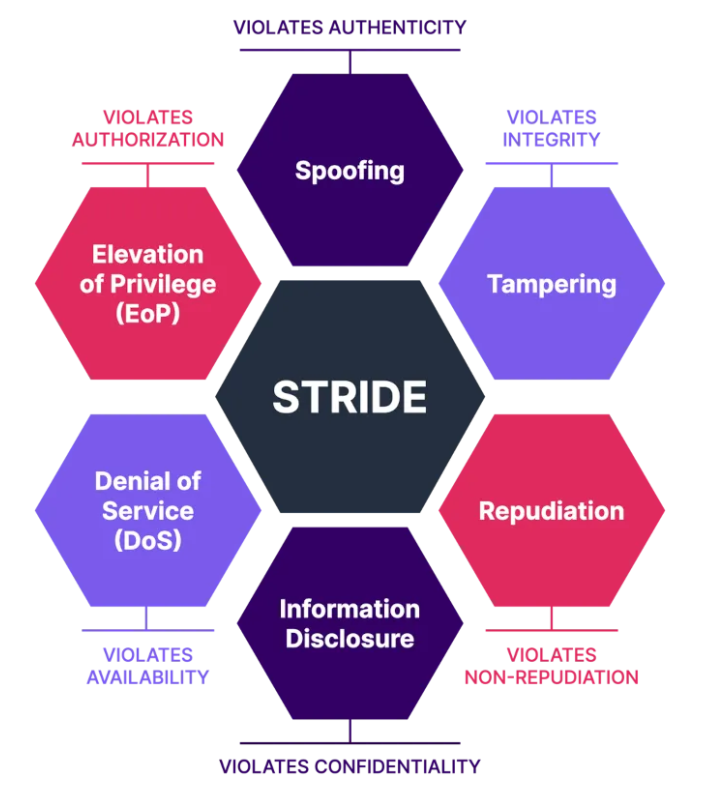
\includegraphics[width=0.5\linewidth]{STRIDE.png}
	\caption{The STRIDE model summarized, illustration from \cite{STRIDE_For_pay_Medium}}
	\label{fig:STRIDE}
\end{figure}

\subsection{Steps in a STRIDE analysis}

\begin{enumerate}
	\item Tally up assets (inventory)
	\item Prepare a Data Flow Diagram (DFD)
	\item Identify boundaries in the DFD, borders are where level of trust changes
	\item Evaluate STRIDE for each component at each border
	\begin{itemize}
		\item Identify Risk 
		\item Propose Mitigation
	\end{itemize} 
\end{enumerate}


\subsection{Asset Enumeration}
A simplified list of assets on the network is shown in Table\ref{tab:assets}, details such as protocols used and software versions should also be included in a detailed enumeration.

\begin{table}[htp]
	\begin{tabular}{|l|l|lll}
		\cline{1-2}
		\textbf{Item}       & \textbf{Description}                                                             &  &  &  \\ \cline{1-2}
		SmartTV\'s           & Wifi connected, has embedded os, receives updates over port 80/443               &  &  &  \\ \cline{1-2}
		Printer             & Network discoverable on local network (IGMP/M-DNS)                               &  &  &  \\ \cline{1-2}
		KidsGamerPC\'s       & Windows os, no restrictions on traffic                                           &  &  &  \\ \cline{1-2}
		IOT gadgets         & MQTT broker/server connected to internet service                                 &  &  &  \\ \cline{1-2}
		Mobile devices      & Ipdas, phones etc,                                                               &  &  &  \\ \cline{1-2}
		Guests joining Wifi & Kids share wifi passwords with their friends etc.                                &  &  &  \\ \cline{1-2}
		Work PC             & Company issued pc, VPN client                                                    &  &  &  \\ \cline{1-2}
		Router              & Provided by ISP, internal firewall blocks inbound traffic except port 80 and 443 &  &  &  \\ \cline{1-2}
	\end{tabular}
	\caption{Simplified enumeration of assets on the network}
	\label{tab:assets}
\end{table}


\subsection{DFD}
The Data flow diagram is shown in Figure \ref{fig:DFD}, Data inbound is only allowed on TCP port 80 and 443, outbound traffic and traffic on the internal network in not limited. The traffic on the internal network consists of a multitude of data and protocols, IOT devices communicate on their own sub protocols (MQTT, zigbee, bluetooth etc.) with servers connected to the home network.

\begin{figure}[!htp] % Single column :figure	
	\centering
	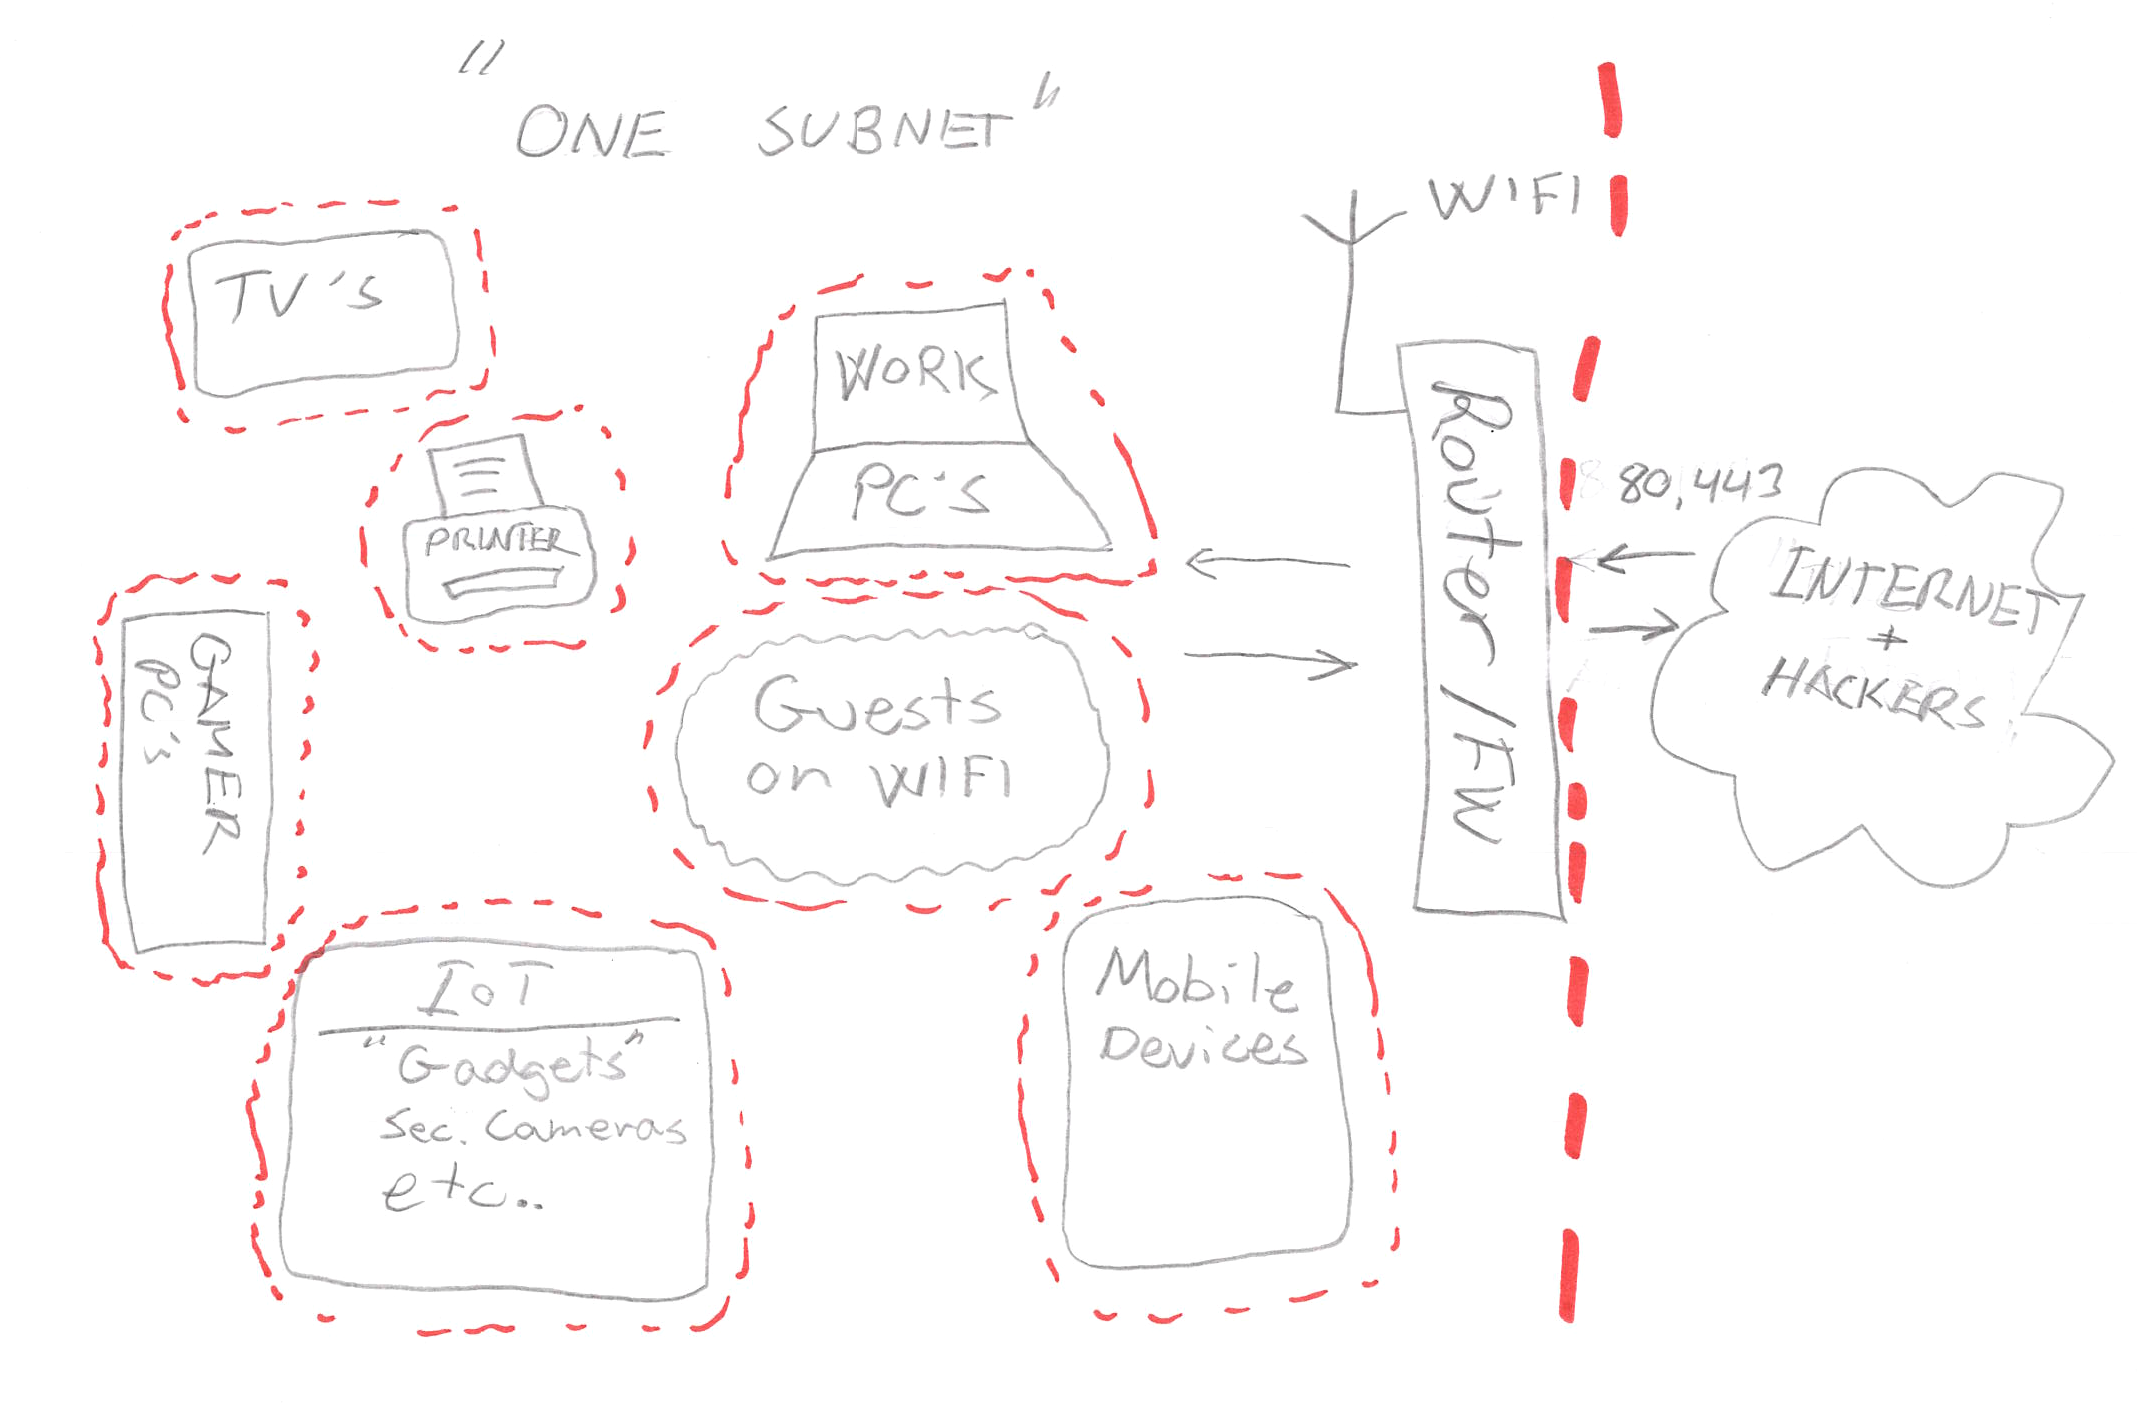
\includegraphics[width=\linewidth]{DFD_home.png}
	\caption{Simple home network Data Flow Diagram, Inbound data only allowed on port 80 and 443, unlimited traffic outbound and on internal subnet}
	\label{fig:DFD}
\end{figure}


\subsection{Boundaries}
Everything on the subnet is un regulated, the main boundary to the internet is blockings all inbound traffic except for TCP port 80 and 443 (red, dashed line in \ref{fig:DFD}), i.e. the main boundary asset is at the router. However, as guests are sometimes allowed onto the it could be argued the they constitute a trust boundary, all the IOT devices, TV's, mobile devices etc, communicates with servers outside the network, receives software updates etc. Therefore each asset is a trust boundary which should be considered (hence the dotted lines around everything.. in Figure \ref{fig:DFD}). 


\section{STRIDE evaluation}
Each asset in Table \ref{tab:assets} is revaluated for each stride. Some of the assets can be lumped together as they share the same STRIDE weakness. 


\subsection{\underline{S}poofing}
\begin{singlespace}

\begin{itemize}
	\item SmartTV\'s
	\item Printer 
	\item IOT gadgets 
\end{itemize}

\subsubsection{Weaknesses:} Un restricted communication on network, if assets are spoofed, it gives the attacker full access to the local network.
\subsubsection{Mitigaiton:} Put devices on a separate network, keep assets software versions updated

\begin{itemize}
	\item KidsGamerPC\'s
\end{itemize}

\subsubsection{Weaknesses:} The pc's are open to the internet with a human in the loop, this gives a indirect access to the local network if e.g. phishing is successful
\subsubsection{Mitigaiton:} Restrict and monitor software on asset, keep endpoint protection (Windows defender) on asset. Possibly move asset to a separate subnet

\begin{itemize}
	\item Guests joining Wifi
\end{itemize}

\subsubsection{Weaknesses:} Wifi passwords may be shared, so anyone can access the private network
\subsubsection{Mitigaiton:} Put guest on a separate subnet (most home routers have this functionality out of the box)

\begin{itemize}
	\item Work PC
\end{itemize}

\subsubsection{Weaknesses:} Asset is protected by a VPN, however if the VPN is spoofed (e.g. by a supply chain attack) the vpn provides a direct access into the local network
\subsubsection{Mitigaiton:} Keep software up to date

\begin{itemize}
	\item Router
\end{itemize}

\subsubsection{Weaknesses:} The router may be spoofed (also partially by spoofing the wifi) someone else may portray to be the router. 
\subsubsection{Mitigaiton:} Keep router firmware up to date, and follow the news if vulnerabilities are found for the asset


\end{singlespace}

\subsection{\underline{T}ampering}
\begin{singlespace}

	\begin{itemize}
		\item SmartTV\'s
		\item Printer 
		\item IOT gadgets 
	\end{itemize}
	
	\subsubsection{Weaknesses:} These often run on outdated firmware and may have security flaws that allow an attacker to tamper with their functionality, potentially turning IoT cameras into surveillance tools for attackers.
	\subsubsection{Mitigaiton:} Put devices on a separate network, keep assets software versions updated
	
	\begin{itemize}
		\item KidsGamerPC\'s
		\item Work pc
		\item Mobile devices
	\end{itemize}
	
	\subsubsection{Weaknesses:} If malware infects devices, attackers can tamper with system files, applications, etc. including exploiting local network access to spread freely
	\subsubsection{Mitigaiton:} Restrict and monitor software on asset, keep endpoint protection (e.g. Windows defender) on asset. Possibly move asset to a separate subnet if possible to protect the local network
	
	\begin{itemize}
		\item Guests joining Wifi
	\end{itemize}
	
	\subsubsection{Weaknesses:} If guests assets are compromised, they may introduce malware to the the local network  
	\subsubsection{Mitigaiton:} Keep guest on a separate network
	
	\begin{itemize}
		\item Router
	\end{itemize}
	
	\subsubsection{Weaknesses:} Configuration settings could be tampered with (if management interfaces are insecure), allowing an attacker to disable protection mechanisms, open ports, or alter routing behavior. Tampering with the firewall could allow an attacker to bypass VPN protections, affecting not only home devices but also the work PC\'s connection to the corporate network.
	\subsubsection{Mitigaiton:} Keep router firmware up to date, and follow the news if vulnerabilities sre found for the asset
	
	
\end{singlespace}
	

\subsection{\underline{R}epudiation}
There are no formal requirements for repudiation on a home network, however if something happens logging is extremely important for trouble shooting and investigation.  

\begin{singlespace}

	\begin{itemize}
		\item SmartTV\'s
		\item Printer 
		\item IOT gadgets 
	\end{itemize}
	
	\subsubsection{Weaknesses:} Not formally required to log anything, but if these assets are compromised and the manufacturer is liable, proof is hard without a log trail. 
	\subsubsection{Mitigaiton:} Do your own logging (advanced), require manufacturer to provide logging.
	
	\begin{itemize}
		\item Router
	\end{itemize}
	
	\subsubsection{Weaknesses:} Most routers do basic logging, e.g. of which assets are connected to the network. If logging is compromised, a bad actor  coud hide on the network
	\subsubsection{Mitigaiton:} Keep router firmware up to date, and follow the news if vulnerabilities sre found for the asset
		
\end{singlespace}


\subsection{\underline{I}nformation disclosure}

\begin{singlespace}

	\begin{itemize}
		\item SmartTV\'s
		\item Printer 
		\item IOT gadgets 
	\end{itemize}
	
	\subsubsection{Weaknesses:} These thing record confidential data e.g. video and audio could disclose sensitive information  
	\subsubsection{Mitigaiton:} Put devices on a separate network, keep assets software versions updated
	
	\begin{itemize}
		\item KidsGamerPC\'s
		\item Work pc
		\item Mobile devices
	\end{itemize}
	
	\subsubsection{Weaknesses:} Personal information, viewing habits, or sensitive data from apps could be exposed, particularly if devices communicate with external servers insecurely. If the VPN connection or the endpoint is insecure, an attacker might capture sensitive traffic or exploit vulnerabilities to extract confidential information.

	\subsubsection{Mitigaiton:} Restrict and monitor software on asset, keep endpoint protection (e.g. Windows defender) on asset. Possibly move asset to a separate subnet if possible to protect the local network

	\begin{itemize}
		\item Router
	\end{itemize}
	
	\subsubsection{Weaknesses:} If the router or firewall is misconfigured or compromised, network traffic (including passwords or personal data) could be disclosed to attackers. Disabling SSL/TLS inspection may also lead to information leakage.
	\subsubsection{Mitigaiton:} Keep router firmware up to date, and follow the news if vulnerabilities sre found for the asset, do not disable security measures
	
	
\end{singlespace}


\subsection{\underline{D}enial os service}
\begin{singlespace}

	\begin{itemize}
		\item SmartTV\'s
		\item IOT gadgets 
	\end{itemize}
	
	\subsubsection{Weaknesses:} These could be made unavailable by resource exhaustion or being overwhelmed by malicious traffic, rendering them unusable.
	\subsubsection{Mitigaiton:} Put devices on a separate network, keep assets software versions updated
	
	\begin{itemize}
		\item WorkPC
	\end{itemize}
	
	\subsubsection{Weaknesses:} Attackers could target the work PC to disconnect it from the corporate network, potentially causing a loss of productivity. This could be done by overloading the VPN connection with traffic incentivizeing user to bypass the VPN making traffic insecure.
	\subsubsection{Mitigaiton:} Have patience, report the incident using a separate channel and do not bypass the VPN

	\begin{itemize}
		\item Router
	\end{itemize}
	
	\subsubsection{Weaknesses:} Attackers could flood the network with traffic (DDoS) to overwhelm the router or firewall, causing loss of internet access.
	\subsubsection{Mitigaiton:} Keep router firmware up to date, and follow the news if vulnerabilities sre found for the asset, do not disable security measures.
	
	
\end{singlespace}



\subsection{\underline{E}levation of privilege} 







\section{Conclusion}
Highly recommend using a tool for this..
There is a lot of copy-pasting, and the tools to do the analysis often end up with 'consultant' flavor to it, where everything is covered but conclusions are difficult to identify. Hence you need to know what you are analyzing to produce a usable analysis result.


%----------------------------------------------------------------------------------------
%	 REFERENCES
%----------------------------------------------------------------------------------------
\clearpage
\printbibliography % Output the bibliography

%----------------------------------------------------------------------------------------



%----------------------------------------------------------------------------------------
%	 Appendices
%----------------------------------------------------------------------------------------

\appendix


\clearpage
\chapter{Appendices}
\begin{appendices}

\end{appendices}
\end{document}
